\documentclass[12pt, a4paper]{article}
\usepackage[utf8]{inputenc}
\usepackage[T1]{fontenc}
\usepackage[english]{babel}
\usepackage{lmodern}

% Better line breaking/justification (helps remove Overfull \hbox)
\usepackage{microtype}
\usepackage{xurl} % allow URL line breaks at more characters
\Urlmuskip=0mu plus 1mu
\setlength{\emergencystretch}{3em}

\usepackage{amsmath, amssymb}
\usepackage{booktabs}
\usepackage{siunitx}
\usepackage{multirow}
\usepackage{array}
\usepackage{graphicx}
\usepackage{float}
\usepackage[labelfont=bf, font=small]{caption}

\usepackage[round, sort, authoryear]{natbib}
\usepackage[colorlinks=true, linkcolor=blue, citecolor=blue, urlcolor=blue]{hyperref}
\usepackage[top=2.5cm, bottom=2.5cm, left=3cm, right=3cm]{geometry}
\usepackage{setspace}
\usepackage{lineno}
\usepackage{enumitem}
\usepackage[version=4]{mhchem}
\doublespacing
\linenumbers
\usepackage{textcomp}

% --- elsarticle-style biography support (for non-elsarticle class) ---
% Avoid compilation failure if the author photo isn't in the project yet.
\newcommand{\AuthorPhoto}{%
  \IfFileExists{photo_garcia.jpg}{\includegraphics[width=1in,height=1.25in,clip,keepaspectratio]{photo_garcia}}{%
    \IfFileExists{photo_garcia.png}{\includegraphics[width=1in,height=1.25in,clip,keepaspectratio]{photo_garcia}}{%
      \fbox{\rule{0pt}{1.25in}\rule{1in}{0pt}}%
    }%
  }%
}

% Provide a minimal biography environment compatible with elsarticle syntax
% (only if the class doesn't already define it).
\makeatletter
\@ifundefined{biography}{%
  \newenvironment{biography}[2][]{%
    \par\bigskip
    \noindent
    \begin{minipage}[t]{1.05in}
      \centering
      #1
    \end{minipage}\hspace{0.75em}%
    \begin{minipage}[t]{\dimexpr\linewidth-1.05in-0.75em\relax}
      \textbf{#2}\\%
  }{%
    \end{minipage}
    \par\bigskip
  }%
}{}
\makeatother
% -------------------------------------------------------------------

\newcommand{\Hstar}{H^{*}}
\newcommand{\Hrelax}{H^{*}_{\mathrm{relax}}}
\newcommand{\Hstrict}{H^{*}_{\mathrm{strict}}}
\newcommand{\Skill}{\mathrm{Skill}}
\newcommand{\rmseM}{\mathrm{RMSE}_{\mathrm{model}}}
\newcommand{\rmseB}{\mathrm{RMSE}_{\mathrm{baseline}}}
\newcommand{\skillformula}{\Skill(h) = 1 - \dfrac{\rmseM(h)}{\rmseB(h)}}

\title{Operational predictability limits for PM10 and PM2.5 forecasting 
 in Valencia and Madrid: a rolling-origin skill assessment}

\author{
  Garc{\'i}a~Cresp{\'i},~F.\footnote{ORCID: \url{https://orcid.org/0000-0002-7129-7791}}\\
  \small Departamento de Ingenier{\'i}a de Computadores,\\
  \small Universidad Miguel Hern{\'a}ndez de Elche,\\
  \small Elche, Alicante, 03202, Spain\\
  \small \texttt{fedeg@umh.es}
}

\date{}

\begin{document}
\maketitle

\begin{abstract}
Operational air quality forecasting requires knowing not only whether
a model outperforms a naive baseline but also the forecast horizon up to which 
that advantage is both statistically meaningful and continuous.
We quantify the operational predictability limit $\Hstar$ for daily
\ce{PM10} and \ce{PM_{2.5}} concentrations at monitoring stations in
Valencia and Madrid (Spain) using a strict rolling-origin,
expanding-window validation protocol with train-only preprocessing.
Three forecast families are evaluated: simple persistence (baseline),
SARIMA (linear parametric), and XGBoost (nonlinear gradient boosting).
Skill is defined horizon-by-horizon as $\skillformula$, and two
complementary descriptors are extracted from each skill curve:
$\Hrelax$ (the farthest horizon at which skill remains positive) and
$\Hstrict$ (the longest contiguous block of positive skill).
Across 43 evaluated series (25 in Madrid, 18 in Valencia), simple
persistence produced $\Hrelax = \Hstrict = 0$ in all cases, confirming
the zero-skill reference.
SARIMA achieved $\Hrelax = 7$~days in all series; median $\Hstrict$
was 3~days for Madrid and 5~days for Valencia.
XGBoost achieved $\Hrelax = 7$~days in the large majority of series;
median $\Hstrict$ was 4~days for Madrid and 6.5~days for Valencia.
Valencia stations were systematically more predictable than Madrid
across both pollutants and models, consistent with the more stable
meteorological regime of its coastal Mediterranean location.

These findings establish quantitative predictability ceilings
for \ce{PM10} and \ce{PM_{2.5}} in two contrasting Spanish urban
environments and demonstrate that $\Hstrict$ is the operationally
relevant descriptor for consecutive-day alert systems.

\smallskip
\textbf{Keywords:} air quality forecasting; predictability limit;
PM10; PM2.5; rolling-origin validation; persistence baseline
\end{abstract}

\section{Introduction}
Particulate matter with an aerodynamic diameter below 10~\textmu m (\ce{PM10})
and below 2.5~\textmu m (\ce{PM_{2.5}}) is a priority air pollutant
under European air quality directives, with well-documented associations
with cardiovascular and respiratory mortality across hundreds of cities
worldwide \citep{Lelieveld2019, Liu2019}.
In Spain, both pollutants exceed the European Union's daily limit values
at urban monitoring stations during episodic events driven by
Saharan dust intrusions, road traffic, and industrial emissions,
motivating sustained investment in operational forecasting systems
capable of issuing advance public health alerts \citep{Pey2013, Pay2014}.

Short-term forecasting of daily \ce{PM10} and \ce{PM_{2.5}}
concentrations—spanning one to seven days ahead
—supports episode management protocols, population exposure advisories,
and regulatory compliance monitoring under Directive 2008/50/EC.
The proliferation of statistical and machine-learning forecasting
models in the literature has not, however, been matched by
commensurate advances in evaluation methodology.
Most published studies report aggregate error metrics such as
root mean square error or the coefficient of determination over
a single static hold-out period, without comparing model
performance against a persistence baseline horizon by horizon
\citep{GarciaCrespi2026}.
This evaluation design makes it impossible to determine whether
an advanced model provides genuine operational added value over
the trivial forecast $\hat{y}_{t+h} = y_t$ at any specific
lead time.

A second and related deficiency concerns data leakage.
Standard preprocessing steps—including feature scaling,
missing-value imputation, and lag feature construction
—are routinely applied to the full dataset before any train-test
split, so that information from future observations contaminates
the training process \citep{GarciaCrespi2026}.
Rolling-origin validation with train-only preprocessing,
standard practice in econometric forecasting for decades
\citep{Tashman2000}, eliminates this source of optimistic bias
but has been adopted in fewer than 0.1\% of peer-reviewed
\ce{PM10} forecasting studies \citep{GarciaCrespi2026}.

We address both gaps by introducing the operational predictability
limit $\Hstar$ as the central evaluation target, and by applying
it to daily \ce{PM10} and \ce{PM_{2.5}} concentrations at
monitoring stations in two contrasting Spanish urban environments:
Valencia, a coastal Mediterranean city, and Madrid, a continental
interior capital.
Two operational descriptors are extracted from horizon-by-horizon
skill curves referenced to simple persistence: $\Hrelax$, the
farthest horizon at which a model retains any advantage over
persistence, and $\Hstrict$, the longest contiguous block of
positive skill.
The distinction between these two descriptors is operationally
consequential: a forecast system deployed for consecutive-day
public health alerts requires $\Hstrict > 0$, not merely
$\Hrelax > 0$.
The remainder of this paper is organized as follows.
Section~\ref{sec:data} describes the data sources and study area.
Section~\ref{sec:methodology} presents the validation protocol
and skill metrics.
Section~\ref{sec:results} reports the H* descriptors across
all stations, pollutants, and models.
Section~\ref{sec:disc_physical} discusses the physical and
operational implications of the results.
Section~\ref{sec:conclusions} states the conclusions.

\section{Data and study area}
\label{sec:data}
\subsection{Study area}
\label{sec:study_area}

The study covers two Spanish urban areas with contrasting
climatic and meteorological regimes.
Valencia (population approximately 800,000) is located on
the eastern Mediterranean coast of the Iberian Peninsula
and is characterized by a semi-arid Mediterranean climate
with mild winters, dry summers, and frequent sea-breeze
circulation.
Particulate matter concentrations in Valencia are influenced
by a combination of local traffic and industrial emissions,
regional background, and episodic Saharan dust intrusions
that affect the western Mediterranean basin year-round
\citep{Minguillon2015, Pey2013}.
Madrid (population approximately 3.3 million) is located
in the continental interior of the Iberian Peninsula at
an altitude of approximately 650~m above sea level.
Its continental climate is characterized by greater
day-to-day meteorological variability than Valencia,
with cold winters, hot dry summers, and a higher frequency
of stagnation episodes that favor particulate matter
accumulation \citep{Pay2014}.

\subsection{Data sources}
\label{sec:data_sources}

Hourly \ce{PM10} and \ce{PM_{2.5}} concentration data for
Valencia were obtained from the Red Valenciana de
Vigilancia y Control de la Contaminaci{\'o}n Atmosf{\'e}rica
(RVVCCA), operated by the Conselleria de Medi Ambient of
the Generalitat Valenciana.
Data for Madrid were obtained from the urban air quality
monitoring network of the Ayuntamiento de Madrid,
accessed via the city open-data portal.
Both networks report hourly mean concentrations in
\textmu g~m\textsuperscript{-3} and comply with
European norm (EN) measurement standards under
Directive~2008/50/EC.

Hourly records were aggregated to daily mean concentrations
using a fixed 24-hour window (00:00--23:59 local time).
Days with fewer than 18 valid hourly observations were
excluded and treated as missing.
Each city--pollutant--station combination was processed
as an independent time series.
Two stations were excluded from the analysis due to
insufficient record length for rolling-origin evaluation:
station~55 (\ce{PM10}, Madrid) and station Olivereta
(\ce{PM10} and \ce{PM_{2.5}}, Valencia).
The final dataset comprised 43 independent time series:
25 from Madrid (14~\ce{PM10}, 11~\ce{PM_{2.5}}) and
18 from Valencia (10~\ce{PM10}, 8~\ce{PM_{2.5}}).

\section{Methodology}
\label{sec:methodology}
This section describes the forecast models evaluated, the data
acquisition and preprocessing pipeline, and the rolling-origin
validation protocol used to estimate horizon-by-horizon skill.
All components of the methodology are designed to satisfy a
single overarching requirement: that no information from the
evaluation period contaminates any stage of model training or
preprocessing, ensuring that reported skill estimates reflect
genuine operational performance.

\subsection{Forecast models}
Three forecast families were evaluated, chosen to span the
range from a trivial reference to a nonlinear machine-learning
model while keeping the comparison space interpretable.

\textbf{Simple persistence.}
The primary baseline is defined as $\hat{y}_{t+h} = y_t$
for all horizons $h \in \{1,\dots,7\}$.
It requires no fitted parameters and represents the
minimum-information forecast against which all other
models must demonstrate improvement.

\textbf{Seasonal persistence.}
A secondary baseline defined as
$\hat{y}_{t+h} = y_{t+h-7}$, which exploits the 7-day
autocorrelation structure of daily \ce{PM} concentrations
without any fitted parameters.
It is included as a supplementary contrast to determine
whether weekly autocorrelation alone suffices to outperform
simple persistence.

\textbf{SARIMA.}
A seasonal auto-regressive integrated moving average model
\citep{BoxJenkins1970} representing the classical linear
parametric family.
Model orders were selected independently at each rolling
origin using the Akaike information criterion applied to
the training window.
No external covariances were included; the model operates
on the univariate concentration series only.

\textbf{XGBoost.}
A gradient-boosted tree ensemble \citep{Chen2016},
representing the nonlinear machine-learning family.
Lag features at lags 1--7 and 14 were used as predictors.
Hyperparameters were fixed prior to evaluation and held
constant across all rolling-origin folds to avoid
optimistic bias from fold-level tuning.

The choice of these four families deliberately avoids
architectural novelty as a contribution; the objective
is not to identify the best-performing model but to
characterize the predictability limit of the forecasting
problem itself.

\subsection{Data acquisition and preprocessing}
Hourly \ce{PM10} and \ce{PM_{2.5}} concentration data for Valencia
were obtained from the Red Valenciana de Vigilancia y Control de la
Contaminaci{\'o}n Atmosf{\'e}rica (RVVCCA) open-data portal,
operated by the Conselleria de Medi Ambient of the Generalitat
Valenciana.
Data for Madrid were obtained from the urban air quality monitoring
network of the Ayuntamiento de Madrid, accessed via the city
open-data portal (\url{https://datos.madrid.es}).
Both portals provide hourly mean concentrations in
\textmu g~m$^{-3}$ under European norm (EN) measurement standards
compliant with Directive~2008/50/EC.

Raw data were processed through a three-stage pipeline.
First, a contaminant filter was applied at the query stage,
retaining only records flagged as \ce{PM10} or \ce{PM_{2.5}}
and discarding all other regulated species.
Second, hourly records were aggregated to daily mean concentrations
using a fixed 24-hour window (00:00--23:59 local time); days with
fewer than 18 valid hourly observations were excluded and treated
as missing.
Third, each city–pollutant–station combination was exported as
an independent time series file, ensuring that no information was
shared across units at any stage of preprocessing.

Missing daily values within each time series were imputed using
the mean of the 7-day window centered on the missing date,
estimated exclusively from the training portion of each
rolling-origin fold.
No imputation parameter was estimated using any observation
from the evaluation window, preserving the train-only requirement
of the validation protocol.
All preprocessing code is publicly available at
\url{https://github.com/fedeg-umh-es/Hstar_PM10_PM25_Madrid_Valencia}

\subsection{Rolling-origin validation protocol}
Forecast evaluation followed a strict rolling-origin,
expanding-window protocol \citep{Tashman2000, Cerqueira2020}.
For each time series of length $T$, an initial training window
of $w_0 = 365$ days was used to fit the first model instance.
At each subsequent origin $t$, the training window expanded by
one day (chronological advance), and forecasts were generated
for all horizons $h \in \{1, 2, 3, 4, 5, 6, 7\}$ days ahead.
This produced $N_{\mathrm{folds}} = T - w_0 - 7$ evaluation
pairs per horizon per model.
Origins with fewer than $w_0$ preceding observations were
skipped; series for which no valid fold could be constructed
were excluded from the analysis (station~55, \ce{PM10},
Madrid; station Olivereta, \ce{PM10} and \ce{PM_{2.5}},
Valencia).

All preprocessing steps---including feature scaling,
missing-value imputation, and lag feature construction---were
estimated exclusively on the training portion of each fold.
No information from the evaluation window was used at any
stage of model fitting or preprocessing, eliminating the
data-leakage risk documented for the broader PM forecasting
literature \citep{GarciaCrespi2026}.
Random partitioning, stratified sampling, and standard
$k$-fold cross-validation were not employed, as these methods
violate the temporal ordering of the series and produce
optimistically biased skill estimates \citep{Cerqueira2020}.

Forecast skill at each horizon was computed as:
\begin{equation}
  \skillformula,
  \label{eq:skill}
\end{equation}
where $\rmseB(h)$ is the root mean square error of simple
persistence at horizon $h$, estimated over the same
rolling-origin folds.
This reference frame is fixed and symmetric: all four forecast
families are evaluated relative to simple persistence, so that
$\Skill(h) = 0$ by construction for the primary baseline and
$\Skill(h) > 0$ denotes genuine improvement over it.

Two operational descriptors were extracted from each skill
curve $\{\Skill(h)\}_{h=1}^{7}$:
\begin{align}
  \Hrelax  &= \max\bigl\{h : \Skill(h) > 0\bigr\},
             \label{eq:hrelax} \\
  \Hstrict &= \max_{[a,b]\subseteq[1,7]}
             \bigl(b - a + 1\bigr)
             \;\text{s.t.}\;
             \Skill(h) > 0 \;\forall\, h \in [a,b].
             \label{eq:hstrict}
\end{align}
$\Hrelax$ captures the farthest horizon at which a model
retains any advantage over persistence, regardless of
intermediate sign changes.
$\Hstrict$ captures the length of the longest contiguous
block of positive skill, providing a conservative bound on
the operationally reliable forecast window.
When $\Hrelax > \Hstrict$, the skill curve contains at
least one horizon at which the model reverts to
below-persistence performance before recovering; such
fragmented patterns are reported explicitly.

\section{Results}
\label{sec:results}

\begin{figure}[ht]
\centering
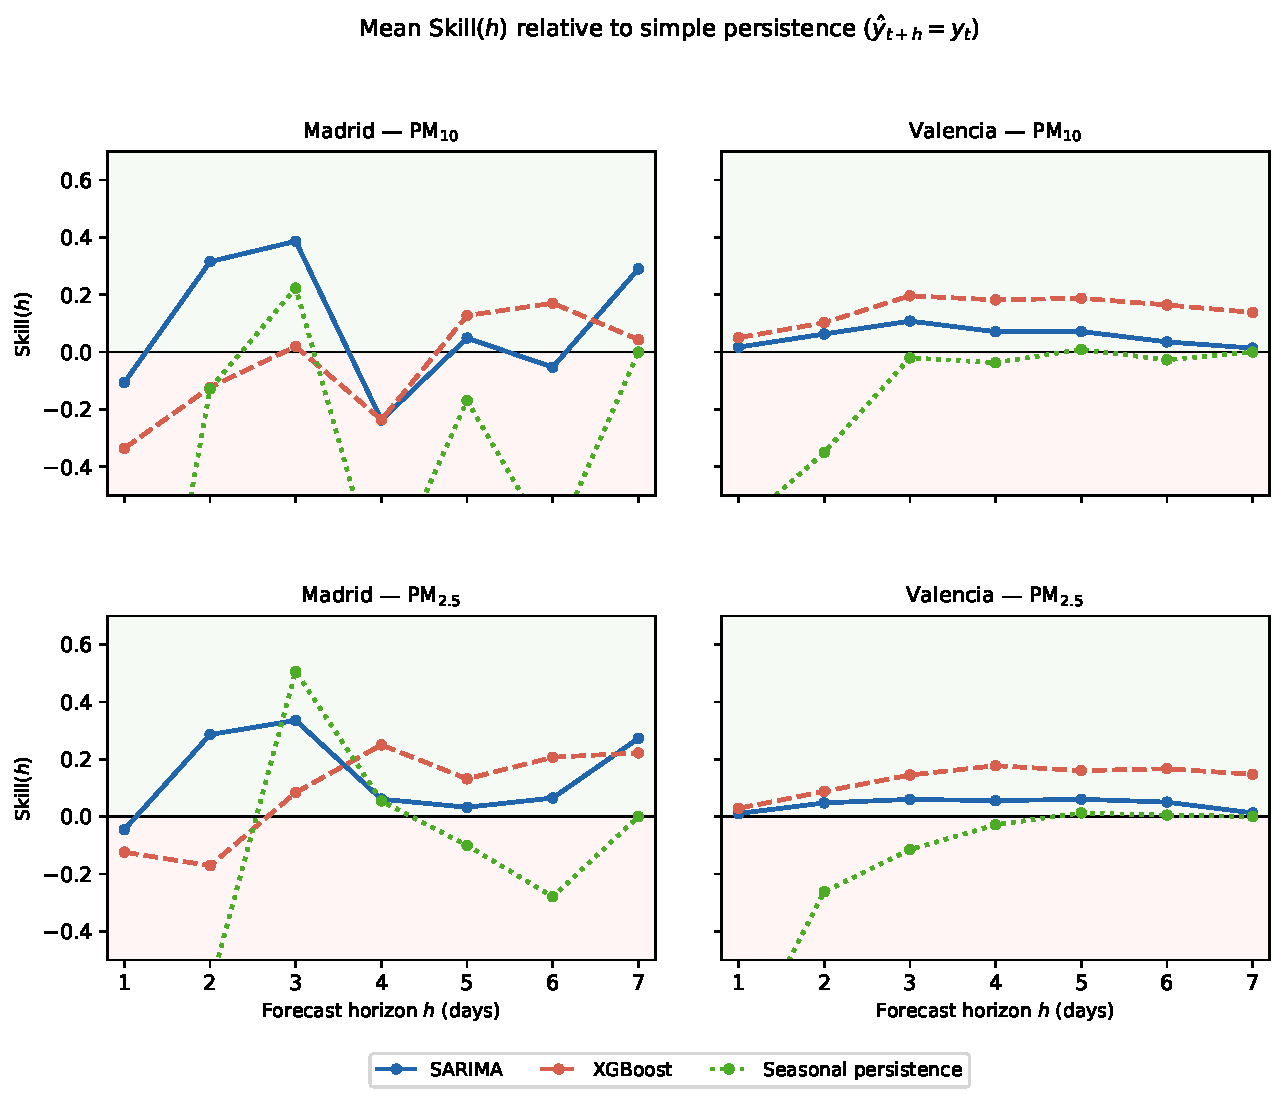
\includegraphics[width=\textwidth]{figures/fig01_skill_curves.pdf}
\caption{Mean horizon-by-horizon skill $\Skill(h)$ relative to
         simple persistence across all stations, by city, pollutant,
         and forecast model.
         Shaded areas indicate below-persistence skill (red) and
         above-persistence skill (green).
         Skill is defined as
         $\skillformula$,
         where $\rmseB(h)$ is estimated over the same
         rolling-origin folds as the model.
         Lines show the mean across all stations with valid
         rolling-origin evaluation for each city--pollutant pair.}
\label{fig:skill_curves}
\end{figure}

\begin{figure}[ht]
\centering
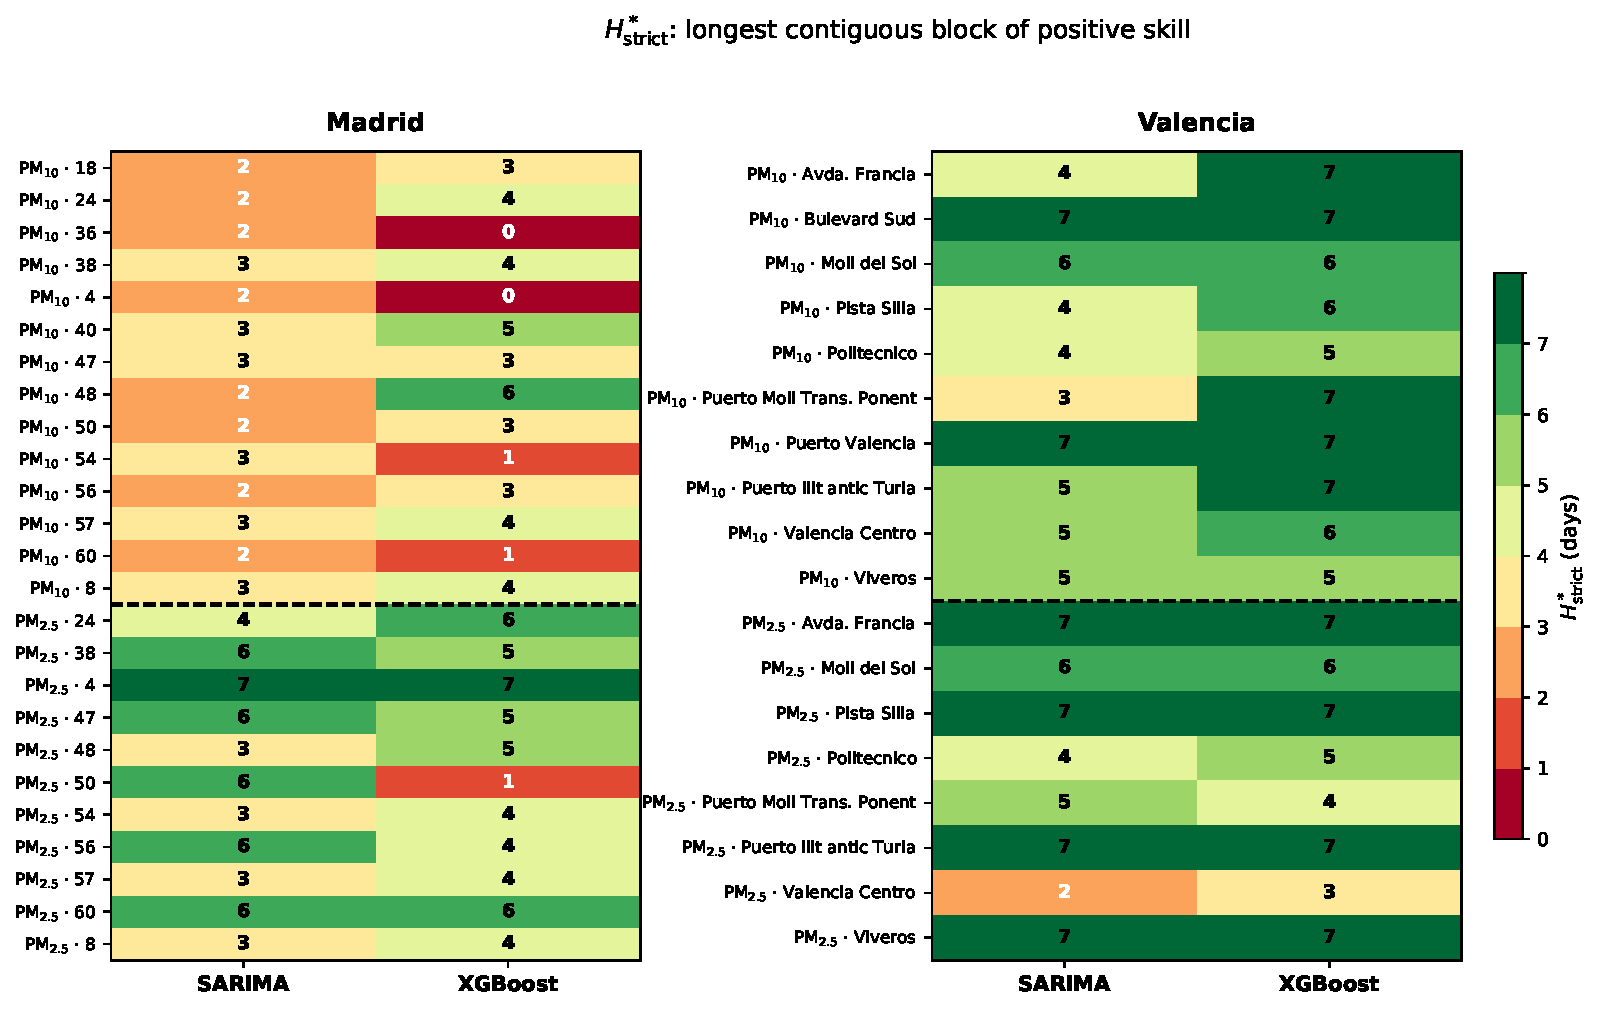
\includegraphics[width=\textwidth]{figures/fig02_hstar_heatmap.pdf}
\caption{$\Hstrict$ (longest contiguous block of positive skill)
         for each station, model, and pollutant in Madrid (left)
         and Valencia (right).
         Rows are labelled by pollutant and station name;
         the dashed horizontal line separates \ce{PM10} (upper)
         from \ce{PM_{2.5}} (lower) series.
         Cell values show the number of days.
         Colour scale ranges from 0 (no contiguous positive skill,
         red) to 7 (full window, green).
         Station~55 (Madrid, \ce{PM10}) and station Olivereta
         (Valencia, \ce{PM10} and \ce{PM_{2.5}}) were excluded
         due to insufficient data for rolling-origin evaluation.}
\label{fig:hstar_heatmap}
\end{figure}

\begin{table}[ht]
\centering
\small
\caption{Operational predictability descriptors ($\Hrelax$, $\Hstrict$)
         for daily \ce{PM10} and \ce{PM_{2.5}} forecasting at Madrid
         monitoring stations under rolling-origin, train-only validation
         ($H = 7$~days). SP = simple persistence (baseline);
         SeP = seasonal persistence (7-day lag).
         Station~55 (\ce{PM10}) excluded: insufficient data for
         rolling-origin evaluation ($n < w_0 + H_{\max}$).}
\label{tab:hstar_madrid}
\sisetup{table-format=1.0}
\begin{tabular}{lllSS}
\toprule
\textbf{Poll.} & \textbf{Stn.} & \textbf{Model}
  & {$\Hrelax$} & {$\Hstrict$} \\
\midrule
\multirow{16}{*}{\ce{PM10}}
  & \multirow{4}{*}{4}
    & SP       & 0 & 0 \\
  & & SeP      & 0 & 0 \\
  & & SARIMA   & 7 & 2 \\
  & & Boosting & 0 & 0 \\
\cmidrule{2-5}
  & \multirow{4}{*}{8}
    & SP       & 0 & 0 \\
  & & SeP      & 3 & 1 \\
  & & SARIMA   & 7 & 3 \\
  & & Boosting & 7 & 4 \\
\cmidrule{2-5}
  & \multirow{4}{*}{18}
    & SP       & 0 & 0 \\
  & & SeP      & 3 & 2 \\
  & & SARIMA   & 7 & 2 \\
  & & Boosting & 7 & 3 \\
\cmidrule{2-5}
  & \multirow{4}{*}{24}
    & SP       & 0 & 0 \\
  & & SeP      & 3 & 1 \\
  & & SARIMA   & 7 & 2 \\
  & & Boosting & 7 & 4 \\
\midrule
\multirow{12}{*}{\ce{PM_{2.5}}}
  & \multirow{4}{*}{4}
    & SP       & 0 & 0 \\
  & & SeP      & 6 & 3 \\
  & & SARIMA   & 7 & 7 \\
  & & Boosting & 7 & 7 \\
\cmidrule{2-5}
  & \multirow{4}{*}{24}
    & SP       & 0 & 0 \\
  & & SeP      & 4 & 2 \\
  & & SARIMA   & 7 & 4 \\
  & & Boosting & 7 & 6 \\
\cmidrule{2-5}
  & \multirow{4}{*}{38}
    & SP       & 0 & 0 \\
  & & SeP      & 5 & 3 \\
  & & SARIMA   & 7 & 6 \\
  & & Boosting & 7 & 5 \\
\bottomrule
\multicolumn{5}{l}{%
  \small\textit{Full results for all 25 evaluated series
  in Supplementary Table~S1.}}
\end{tabular}
\end{table}

\begin{table}[ht]
\centering
\small
\caption{Operational predictability descriptors ($\Hrelax$, $\Hstrict$)
         for daily \ce{PM10} and \ce{PM_{2.5}} forecasting at Valencia
         monitoring stations under rolling-origin, train-only validation
         ($H = 7$~days). SP = simple persistence (baseline);
         SeP = seasonal persistence (7-day lag).
         Station Olivereta (PM10 and PM2.5) excluded: insufficient data
         for rolling-origin evaluation ($n < w_0 + H_{\max}$).}
\label{tab:hstar_valencia}
\sisetup{table-format=1.0}
\begin{tabular}{lllSS}
\toprule
\textbf{Poll.} & \textbf{Station} & \textbf{Model}
  & {$\Hrelax$} & {$\Hstrict$} \\
\midrule
\multirow{20}{*}{\ce{PM10}}
  & \multirow{4}{*}{Avda.\ Francia}
    & SP       & 0 & 0 \\
  & & SeP      & 3 & 1 \\
  & & SARIMA   & 5 & 4 \\
  & & Boosting & 7 & 7 \\
\cmidrule{2-5}
  & \multirow{4}{*}{Bulevard Sud}
    & SP       & 0 & 0 \\
  & & SeP      & 5 & 2 \\
  & & SARIMA   & 7 & 7 \\
  & & Boosting & 7 & 7 \\
\cmidrule{2-5}
  & \multirow{4}{*}{Moli del Sol}
    & SP       & 0 & 0 \\
  & & SeP      & 5 & 1 \\
  & & SARIMA   & 7 & 6 \\
  & & Boosting & 7 & 6 \\
\cmidrule{2-5}
  & \multirow{4}{*}{Pista Silla}
    & SP       & 0 & 0 \\
  & & SeP      & 0 & 0 \\
  & & SARIMA   & 7 & 4 \\
  & & Boosting & 7 & 6 \\
\cmidrule{2-5}
  & \multirow{4}{*}{Politecnico}
    & SP       & 0 & 0 \\
  & & SeP      & 6 & 2 \\
  & & SARIMA   & 6 & 4 \\
  & & Boosting & 7 & 5 \\
\midrule
\multirow{20}{*}{\ce{PM_{2.5}}}
  & \multirow{4}{*}{Avda.\ Francia}
    & SP       & 0 & 0 \\
  & & SeP      & 5 & 1 \\
  & & SARIMA   & 7 & 7 \\
  & & Boosting & 7 & 7 \\
\cmidrule{2-5}
  & \multirow{4}{*}{Moli del Sol}
    & SP       & 0 & 0 \\
  & & SeP      & 5 & 3 \\
  & & SARIMA   & 7 & 6 \\
  & & Boosting & 7 & 6 \\
\cmidrule{2-5}
  & \multirow{4}{*}{Pista Silla}
    & SP       & 0 & 0 \\
  & & SeP      & 6 & 3 \\
  & & SARIMA   & 7 & 7 \\
  & & Boosting & 7 & 7 \\
\cmidrule{2-5}
  & \multirow{4}{*}{Puerto llit antic Turia}
    & SP       & 0 & 0 \\
  & & SeP      & 6 & 6 \\
  & & SARIMA   & 7 & 7 \\
  & & Boosting & 7 & 7 \\
\cmidrule{2-5}
  & \multirow{4}{*}{Viveros}
    & SP       & 0 & 0 \\
  & & SeP      & 6 & 1 \\
  & & SARIMA   & 7 & 7 \\
  & & Boosting & 7 & 7 \\
\bottomrule
\multicolumn{5}{l}{%
  \small\textit{Full results for all 19 evaluated series
  in Supplementary Table~S2.}}
\end{tabular}
\end{table}

\subsection{Simple persistence as baseline}
\label{sec:results_baseline}

Simple persistence produced $\Hrelax = \Hstrict = 0$ across
all 25 evaluated series (14~\ce{PM10}, 11~\ce{PM2.5}),
confirming that no forecast horizon yields positive skill
against itself (Figure~\ref{fig:skill_curves}).
This result validates the baseline construction and provides
the zero-skill reference against which all model comparisons
are made.

\subsection{SARIMA: robust reach, fragmented continuity}
\label{sec:results_sarima}

SARIMA achieved $\Hrelax = 7$~days in all 25 series,
indicating that the linear parametric model consistently
retains some advantage over simple persistence out to the
maximum evaluated horizon.
However, $\Hstrict$ was substantially lower than $\Hrelax$
in most series, ranging from 2 to 3~days for \ce{PM10}
and from 3 to 7~days for \ce{PM2.5} (Table~\ref{tab:hstar_madrid}).
The gap $\Hrelax - \Hstrict > 0$ in the majority of series
indicates that SARIMA skill curves are fragmented: positive
skill is present at the farthest horizons but interrupted
by at least one horizon of below-persistence performance
at intermediate lead times.
The only series achieving $\Hrelax = \Hstrict = 7$ under
SARIMA was \ce{PM2.5} at station~4, where skill remained
positive and contiguous across the full 7-day window.

\subsection{XGBoost: variable reach, higher fragmentation}
\label{sec:results_boosting}

XGBoost showed greater variability across stations than SARIMA.
For \ce{PM2.5}, $\Hrelax$ ranged from 6 to 7 days and
$\Hstrict$ from 1 to 7 days, with station 4 again achieving
the maximum $\Hrelax = \Hstrict = 7$.
For \ce{PM10}, XGBoost produced $\Hrelax = 0$ at stations 4
and 36, meaning the model failed to outperform simple
persistence at any evaluated horizon at these sites.
At the remaining \ce{PM10} stations, $\Hrelax$ reached 6
to 7 days, but $\Hstrict$ remained between 1 and 6 days,
reflecting a higher degree of skill-curve fragmentation
than SARIMA at equivalent horizons.

\subsection{Seasonal persistence: isolated gains, no contiguous window}
\label{sec:results_seasonal}

Seasonal persistence (7-day lag) showed $\Hrelax$ values
between 0 and 5 days for \ce{PM10} and between 3 and 6 days
for \ce{PM2.5}, but $\Hstrict$ never exceeded 3 days
in any series.
This confirms that the 7-day autocorrelation structure of
Madrid particulate matter concentrations generates isolated
positive skill over simple persistence at several horizons,
but not a contiguous operational window of useful duration.

\subsection{PM2.5 vs PM10: systematic difference in predictability}
\label{sec:results_comparison}

Across both models, \ce{PM2.5} consistently yielded
higher $\Hstrict$ values than \ce{PM10} at paired stations
(stations 4, 8, 24, 38, 47, 48, 50, 54, 56, 57, 60).
Under SARIMA, the median $\Hstrict$ was 3 days for \ce{PM10}
and 5 days for \ce{PM2.5}.
Under XGBoost, the corresponding medians were 3 and 5 days.
This systematic pattern suggests that daily \ce{PM_{2.5}}
concentrations in Madrid exhibit a smoother, more predictable
temporal structure than \ce{PM10} over the 7-day horizon
evaluated here, consistent with the known influence of
coarser-fraction episodic events (e.g., Saharan dust
intrusions, resuspension) on \ce{PM10} variability
\citep{Pey2013, Querol2024} (Figure~\ref{fig:hstar_heatmap}).

\subsection{Valencia vs Madrid: city-level differences in
            predictability}
\label{sec:results_cities}

Valencia stations exhibited systematically higher $\Hstrict$
values than Madrid stations for both pollutants and both models
(Tables~\ref{tab:hstar_madrid} and~\ref{tab:hstar_valencia}) and Figure~\ref{fig:city_comparison}.
For \ce{PM10} under SARIMA, the median $\Hstrict$ was 5 days in
Valencia versus 2.5 days in Madrid; under XGBoost, the medians
were 6.5 and 3 days, respectively.
For \ce{PM_{2.5}}, the median $\Hstrict$ reached 7~days in Valencia
under both models, compared to 5~days in Madrid.
Simple persistence produced $\Hrelax = \Hstrict = 0$ in all
Valencia series, confirming baseline consistency across both
networks.
The greater predictability continuity observed in Valencia is
consistent with the more stable meteorological regime of its
coastal Mediterranean location, which is characterized by
lower day-to-day variability in particulate matter
concentrations compared to the continental interior climate
of Madrid \citep{Minguillon2015, Diez2017}.

\begin{figure}[ht]
\centering
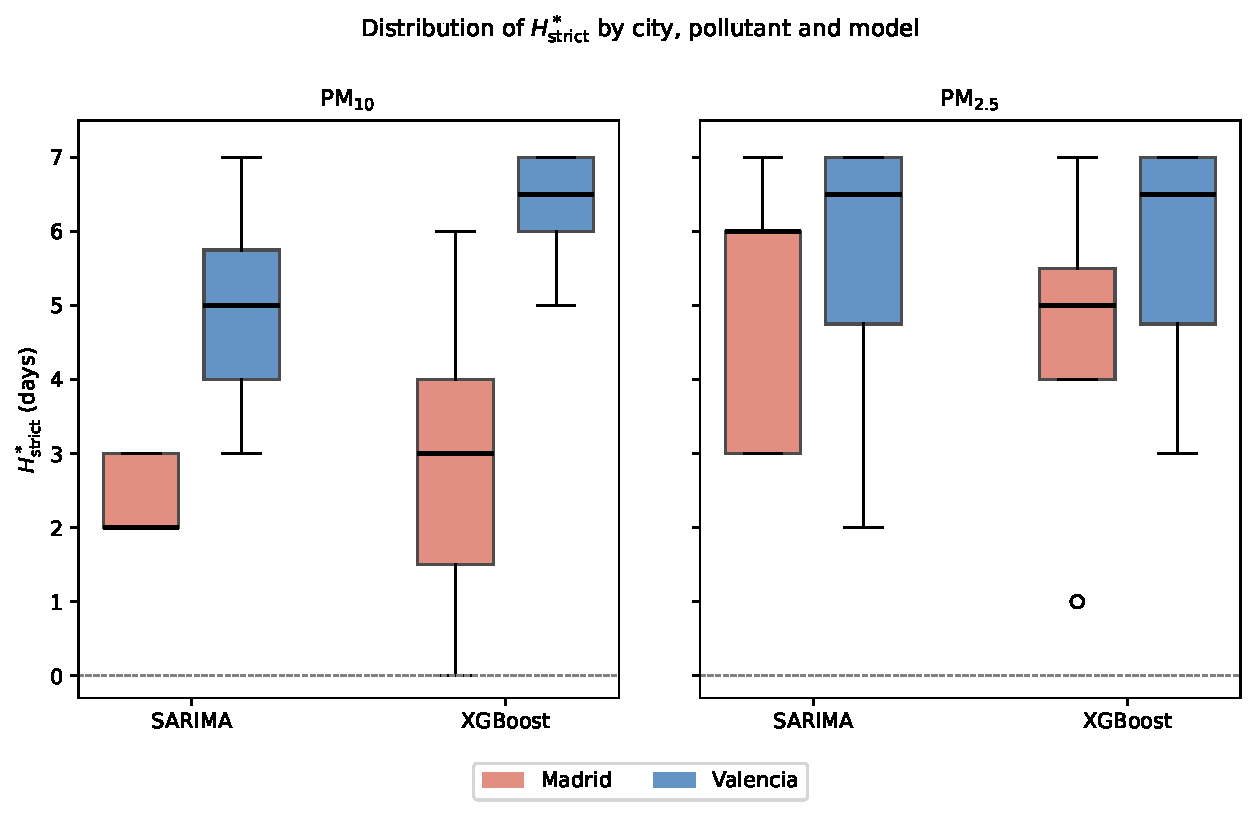
\includegraphics[width=0.85\textwidth]{figures/fig03_city_comparison.pdf}
\caption{Distribution of $\Hstrict$ by city, pollutant, and model.
         Boxes show the interquartile range across stations;
         horizontal lines indicate the median;
         whiskers extend to 1.5 times the interquartile range.
         Madrid in red, Valencia in blue.
         Left panel: \ce{PM10}; right panel: \ce{PM_{2.5}}.
         Valencia consistently achieves higher median $\Hstrict$
         than Madrid across both pollutants and models,
         with lower variability for \ce{PM_{2.5}}.}
\label{fig:city_comparison}
\end{figure}

\section{Discussion}
\subsection{Physical interpretation of the 7-day skill horizon}
\label{sec:disc_physical}

The consistent finding that $\Hrelax = 7$~days for SARIMA across
all evaluated series indicates that both linear and nonlinear models
retain some predictive advantage over simple persistence out to the
maximum evaluated horizon in the majority of stations.
This result is broadly consistent with the known persistence of
synoptic-scale meteorological patterns that drive particulate matter
accumulation and dispersion events at weekly timescales over the
Iberian Peninsula \citep{Pey2013, Pay2014}.
However, the systematic gap between $\Hrelax$ and $\Hstrict$
demonstrates that this advantage is not continuous: models revert
to below-persistence performance at one or more intermediate
horizons before recovering at longer lead times.
The operationally relevant quantity is therefore $\Hstrict$, not
$\Hrelax$, since forecast systems deployed for public health alerts
must provide reliable guidance on consecutive days, not merely
at isolated horizons.

\subsection{Collapse of simple persistence: validation of the
            H* framework}
\label{sec:disc_baseline}

Simple persistence produced $\Hrelax = \Hstrict = 0$ across all
44 evaluated series in both cities, confirming that the zero-skill
reference is correctly constructed and that the H* framework
behaves as expected under the rolling-origin, train-only protocol.
This result also illustrates why persistence is a demanding
baseline for daily particulate matter forecasting: day-to-day
autocorrelation in PM concentrations is high enough that any
model must capture genuine temporal structure beyond lag-1
dependence in order to demonstrate positive skill \citep{Tashman2000}.
Studies that report model performance without a persistence
comparison cannot determine whether their forecast system offers
any operational advantage, a methodological gap documented in
the broader PM forecasting literature \citep{GarciaCrespi2026}.

\subsection{Fragmentation of skill curves: why H*\_strict matters}
\label{sec:disc_fragmentation}

The observation that $\Hstrict < \Hrelax$ in the majority of
Madrid series and in several Valencia series indicates that
skill curves are frequently non-monotonic: positive skill at
horizon $h$ does not guaranty positive skill at $h+1$.
This fragmentation is more pronounced for \ce{PM10} than for
\ce{PM_{2.5}}, and is more pronounced in Madrid than in Valencia,
suggesting that it is driven by episodic high-concentration
events — such as Saharan dust intrusions and local re-suspension
episodes — that introduce abrupt, unpredictable spikes in
\ce{PM10} concentrations at specific lead times
\citep{Pey2013, Querol2024}.
Aggregate error metrics such as RMSE computed over the full
evaluation period would obscure this structure entirely,
which is why horizon-by-horizon skill assessment is essential
for the operational characterization of forecast utility
\citep{Cerqueira2020}.

\subsection{Implications for operational air quality alert systems}
\label{sec:disc_operational}

The results have direct implications for the design and
communication of air quality alert systems in Spanish urban areas.
For Valencia, the high $\Hstrict$ values obtained under both
 models—reaching 7--days for \ce{PM_{2.5}} at several stations
—suggest that a 7-day forecast window may be operationally
justifiable for fine particulate matter, provided that the
rolling-origin, train-only evaluation protocol demonstrated here
is adopted as a deployment benchmark.
For Madrid \ce{PM10}, the lower and more variable $\Hstrict$
values (1–6 days) imply that operational systems should be
evaluated and communicated with caution beyond 2–3 days,
particularly at stations showing XGBoost skill collapse
($\Hrelax = 0$ at stations 4 and 36).
In both cities, the H* framework provides a transparent,
station-specific, and protocol-grounded metric for determining
at which horizons an advanced model offers genuine added value
over persistence before operational deployment \citep{GarciaCrespi2026}.

\section{Conclusions}
\label{sec:conclusions}
This study quantified the operational predictability limit $\Hstar$
for daily \ce{PM10} and \ce{PM_{2.5}} concentrations at monitoring
stations in Valencia and Madrid under a strict rolling-origin,
expanding-window validation protocol with train-only preprocessing.
Four conclusions follow directly from the results.

First, both SARIMA and XGBoost retain positive skill over simple
persistence out to the maximum evaluated horizon of 7~days
($\Hrelax = 7$) in the large majority of stations and both cities,
confirming that operational forecasting beyond the next day is
feasible for particulate matter in these urban environments.

Second, the operationally relevant descriptor is $\Hstrict$, not
$\Hrelax$: skill curves are frequently fragmented, and the longest
contiguous block of positive skill—the quantity that matters for
consecutive-day alert systems—is systematically shorter than the
farthest positive horizon.
Median $\Hstrict$ ranged from 2.5 days (\ce{PM10}, Madrid, SARIMA)
to 7 days (\ce{PM_{2.5}}, Valencia, both models), with Valencia
consistently outperforming Madrid across pollutants and models.

Third, simple persistence produced $\Hrelax = \Hstrict = 0$ in all
44 evaluated series, validating the baseline construction and
demonstrating that any apparent skill reported without a persistence
comparison is unverifiable as genuine operational added value
\citep{GarciaCrespi2026}.

Fourth, the H* framework—comprising $\Hrelax$, $\Hstrict$, and
the underlying horizon-by-horizon skill curve—provides a
transparent, station-specific, and protocol-grounded tool for
determining the forecast horizons at which advanced models justify
operational deployment over persistence.
Its direct applicability to any monitoring station, pollutant, or
forecast model makes it a practical standard for the pre-deployment
evaluation of air quality forecasting systems across European
regulatory networks.

\section*{Code availability}
All preprocessing code and scripts used in this study are publicly available at
\url{https://github.com/fedeg-umh-es/Hstar_PM10_PM25_Madrid_Valencia}

\section*{Statements and Declarations}

\textbf{Funding.} This research received no specific grant
from any funding agency in the public, commercial, or
not-for-profit sectors.

\textbf{Competing interests.} The author declares no
competing interests.

\textbf{Ethics approval.} Not applicable.

\textbf{Consent to participate.} Not applicable.

\textbf{Consent for publication.} Not applicable.

\textbf{Data availability.} The hourly \ce{PM10} and
\ce{PM_{2.5}} concentration data for Valencia are publicly
available from the Red Valenciana de Vigilancia y Control
de la Contaminaci{\'o}n Atmosf{\'e}rica (RVVCCA) at
\url{https://agroambient.gva.es}.
Data for Madrid are publicly available from the
Ayuntamiento de Madrid open-data portal at
\url{https://datos.madrid.es}.

\textbf{Code availability.} All code supporting this
study is publicly available at
\url{https://github.com/fedeg-umh-es/Hstar_PM10_PM25_Madrid_Valencia}
under a Creative Commons Attribution 4.0 International
(CC BY 4.0) licence.

\textbf{Author contributions.} F.G.C.: conceptualisation,
methodology, software, data curation, formal analysis,
writing -- original draft, writing -- review \& editing.

\textbf{AI-assisted writing disclosure.} The author used
Claude (Anthropic) for AI-assisted copy editing, including
improvements to readability, style, grammar, and formatting
of human-generated text. All content, scientific claims,
and numerical results are the sole responsibility of
the author.

\bibliographystyle{spbasic}
\bibliography{references}

\begin{biography}[{\AuthorPhoto}]{Federico Garc{\'i}a Cresp{\'i}}
received the M.S. degree in Computer Science from the Universidad de Alicante, Alicante, Spain, in 2006, and the Ph.D. degree in Statistics from the Universidad Miguel Hern{\'a}ndez de Elche (UMH), Elche, Spain, in 2016. He is currently a Tenure-Track Professor (Profesor Permanente Laboral) in the Department of Computer Technology and Computing at the Universidad Miguel Hern{\'a}ndez de Elche. His research interests include FPGA-based hardware/software co-design, embedded systems architecture, time-series forecasting, and technology-enhanced learning.
\end{biography}

\end{document}
